\pagestyle{empty}
\section{System Testing \\{\small\tt{J.~Pearse}}}
The behaviour of the simulation was verified and tested using a combination of the diagnostic tools integrated into the visualisation, diagnostic functions exported from Erlang modules and prototyping (see section:\ref{pso}). Entity behaviours arising from interactions were observed and investigated (section:\ref{entity_interactions}). The highly concurrent nature of the simulation presents some particular challenges.

\subsection{Simulation reporting}
The major task of compiling a snap-shot of the system state at any given time is handled by the \emph{report} function of the \emph{environment} module this is the function called by the client to update the visualisation \ref{client}.
The function builds a list of entity data gathered sequentially from each tile. Tiles keep details of the states of entities on them so the compiled list contains a snap-shot of all entity states across all tiles. However some time will elapse between the time the environment calls one tile and another.
\begin{enumerate}
\item{environment calls Tile A and adds its state to the report, entities on Tile B are still moving}
\item{environment calls Tile B and concatenates this with the report from tile A, entities on Tile A meanwhile may have moved}
\end{enumerate}
Matters are further complicated by the independent states of entities, before an entity moves it updates its state by calling the viewer to examine its surroundings, then it calls the tile with its updated position (see section:\ref{viewer_intro}, particularly fig:\ref{fig:tile_viewer_communication})  - in the meantime other entities will have called the tile with their updated positions.
Any given report submitted from the environment consists of many entity states, captured at slightly differing times. Although the report has such discrepancies in the data, the simulation itself does not rely on the report data for any function.
\subsection{Visualisation}
Every object drawn in the visualisation uses data from the WebSocket report which is very helpful in understanding the state of the simulation. The SVG format uses a coordinate system with the \( \{ 0,0 \} \) origin in the top-left corner, this same system is used in the simulation internal co-ordinates facilitating the direct mapping of simulation positions to visualisation elements. 
The position values are multiplied with a magnification value for the visualisation, set by the Grid Scale drop-down - here set at \(9\) as we can see arbitrary attributes (such as y\_vel) can be assigned to each element of the SVG. In fig:\ref{fig:co-ordinate mapping} We see the visualisation in its initial state, the system has not started yet, the entity state is largely empty. In the JavaScript console we can examine the SVG element corresponding to the selected entity, we see the X and Y values are equal to the ones in the entity state multiplied by the grid scale value above.
There is animated 'tweening' between reports which sometimes causes the appearance of entities cutting corners in the animation. The speed of individual entities is clearly observable in the visualiser allowing us to see the effect of energy-loss slowing them down gradually and then speeding up again when they gain more energy.
\subsection{Inspection panel}
\label{inspector_panel}
The inspection panel displays elements from the state of any entities selected in the visualiser. By pausing the simulation and clicking on an entity, the process id of the entity can be determined and used to call any exported functions from the Erlang console. The data-binding methods provided by the Angular.js library such as \emph{ng-repeat} allow an html element to be displayed for each item in a JavaScript array, when an entity is clicked in the visualisation it is added to a \emph{display\_list} array, which is simply iterated over and the contents of each element-state is printed in the inspector.
As the inspector panel is dynamically updated the length of the lists of visible entities grows and shrinks causing the entire visualisation to jump erratically up and down the page, the inspector panel can be hidden to stabilise the visualisation. 
\subsection{Line of sight}
\begin{figure}[h]
  \centering
  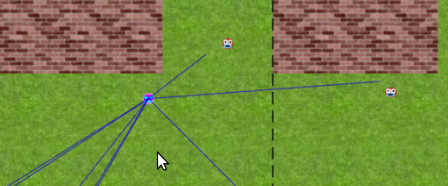
\includegraphics[width=0.5\textwidth]{img/concurrent-lag.png}
\caption{Concurrency visualised}
    \label{fig:Concurrency visualised}
\end{figure}
A line connecting every entity in both the human and zombie lists to the selected entity is drawn into the SVG, (fig:\ref{fig:Concurrency visualised} the interesting aspect of the LOS visualisation is the way it reveals the concurrency inherent in the system, lines are not always drawn to the exact position where entities are, because lines are drawn based on the selected entities state they are sometimes drawn to the position of their target in the previous or next report cycle although this gives the appearance that the visualisation is out of sync, it's a natural effect of trying to visualise a highly concurrent system in discrete snapshots. The fact that lines can be drawn to the position target entities will be in, at the next step of the visualisation gives us evidence that the target entity in question has moved since the report was taken from that tile, i.e. the viewer and hence entity state, have updated during the construction of the report. The entity is drawn at the position reported by the tile when it was called. The subject entity however, is already aware of the targets new location, as the neighbouring tile has updated the viewer.
Consider the following sequence of events:
\begin{enumerate}
\item{tileA and tileB are neighbours so tileA reports its contents to viewerA and vice versa.}
\item{The environment collects a report from tileA, this will be used by the visualisation to draw entity positions and states of entities on this tile.}
\item{A subject on tileA updates its position, causing the viewer of tileB to be updated.}
\item{The environment collects report data from tileB where entity states may now reflect the updated contents of tileA.}
\end{enumerate}
As we can see, although all states were correct at the time of reporting, there is a discrepancy.
\begin{figure}[b]
  \centering
  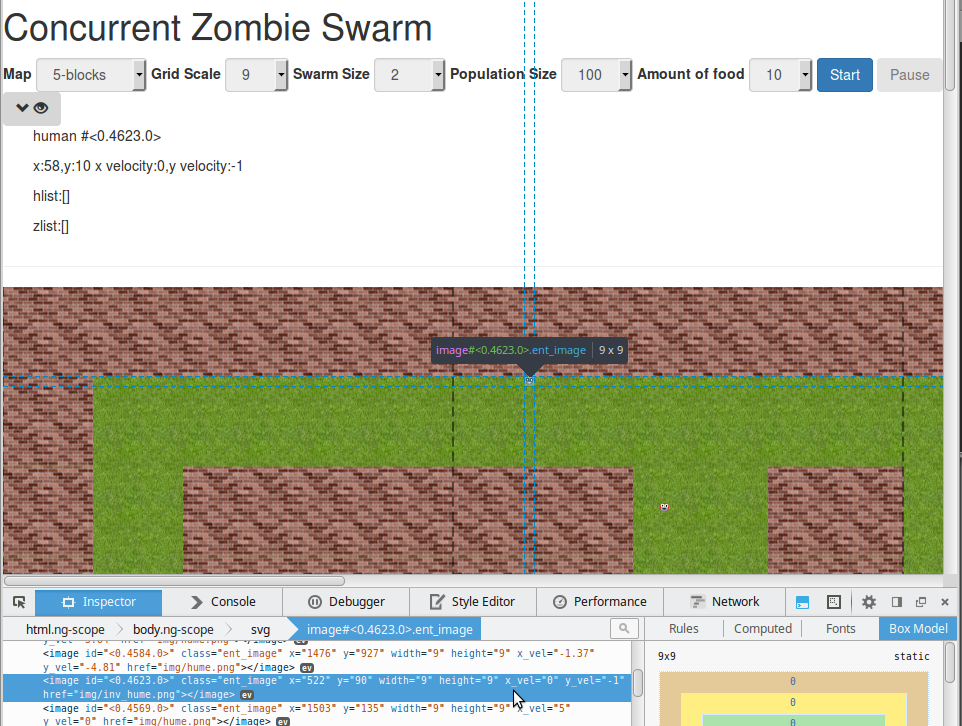
\includegraphics[width=1\textwidth]{img/co-ordinates.png}
\caption{Co-ordinate mapping}
    \label{fig:co-ordinate mapping}
\end{figure}

\clearpage
\endinput
